\chapter{The ATLAS Detector}

The \ac{ATLAS} detector is a cylindrical general purpose particle detector designed to measure the products of $\sqrt{s} = 14 \TeV$ proton-proton collisons at the \ac{LHC}. It consists of three major sub-detectors: closest to the beamline is the the \ac{ID}, which measures the tragectories of charge particles, followed by the Calorimeters, which measure the energies of electromagnetic and hadronically interacting particles, and finally the \ac{MS} which measures the trajectories of muons. The \ac{ID} is surrounded by a super conducting solenoidal magnet that provides a uniform $2\textrm{T}$ magnetic field, enabling measurement of particles' charge and momentum, and a torodial magnet surrounds \ac{MS}, allowing for charge and momentum measurements of muons. A schematic of the \ac{ATLAS} detector is shown in \autoref{fig:atlas-schematic}.


%https://atlas.cern/discover/detector
\begin{figure}[htbp]
\centering
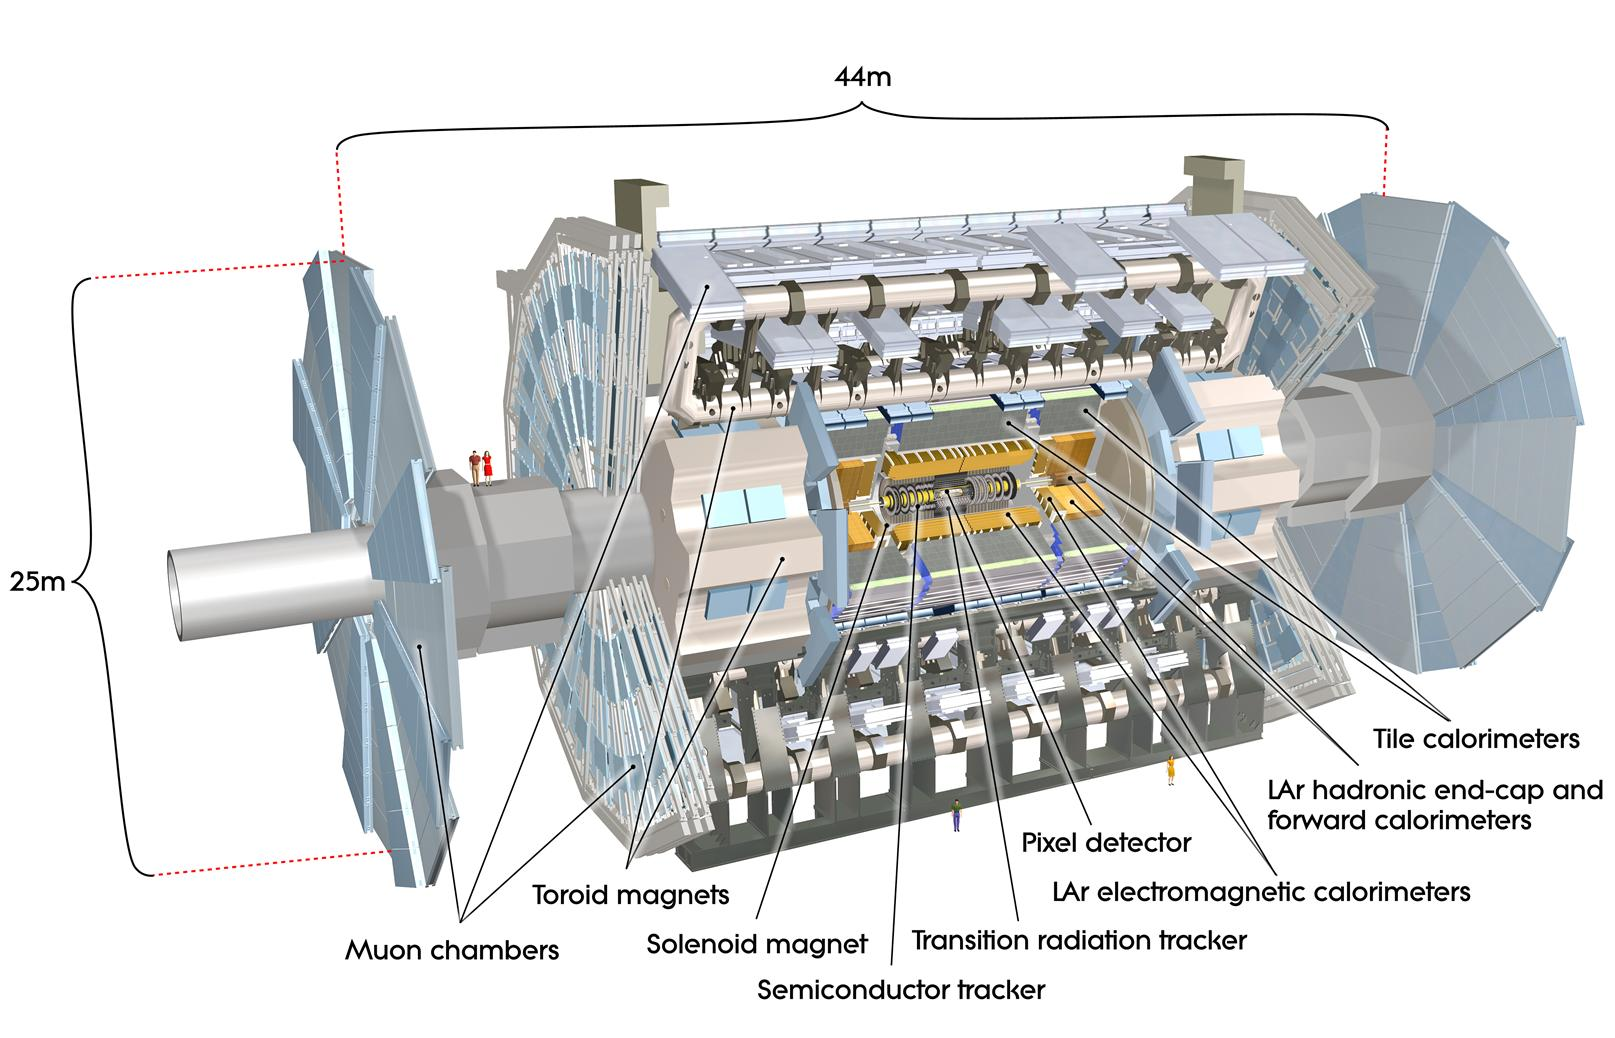
\includegraphics[width=.8\textwidth]{figures/Detector/atlas-schematic.jpg}
\caption{A schematic of the \ac{ATLAS} detector. The dimensions, subdetectors, and magnet systems are labeled. }
\label{fig:atlas-schematic}
\end{figure}

\section{Coordinate System}
\ac{ATLAS} uses a cartesian right-handed coordinate system, with the origin defined as the $pp$ collision point. The $z$-axis points along the beampipe, where $+z$ points counter-clockwise. The transvers plane, the $y$-axis and $x$-axis, points upward and toward the center of the \ac{LHC} ring, respectively. The detector is built with with symmetry across the origin in in $z$, as well as with rotational symmetry in the transverse plane. The $+z$ side of the detector is referred to as the A-side, and $-z$ as the C-side.

Cylindrical coordinates provide a comfortable description of the \ac{ATLAS} detector, where $\phi$ measures the angle in the $x-y$ plane around the beampipe, and $\theta$ the angle from the $z$ axis. $\phi$ is positive for positive $y$. 

A given's particle's momentum in $z$ is not known, but its transverse momentum is known to be $0$, so it is advantageous to define spatial variables independent of $z$ momentum. Thus, instead of $\theta$, $\eta = - \textrm{ln}(\textrm{tan}\frac{\theta}{2})$ is used to describe angle from the $z$ axis. Particles perpindicular to the $z$ axis have $\eta = 0$, while those parallel to the beamline have $\eta \rightarrow \infty$. 

Angular distances between objects is described using $\Delta R = \sqrt{\Delta \eta ^2 + \Delta \phi ^2}$ and the radial distance from the origin in the $x-y$ plane is denoted $R$. 

A particle's momentum will generally be described in terms of its \pT, its momentum in the transverse direction. A particle's $3$-vector is described by $(\pt, \eta, \phi)$, which are all invariant under boosts in $z$ assuming the particle can be considered massless (which is true in the case of particles in \ac{ATLAS}).

\section{Inner Detector}
\section{Calorimeters}
\section{Muon Spectrometer}
\section{Magnet Systems}
\section{Particles in ATLAS}

\todo{describe visible/invisible particles}